\startfirstchapter{Introduction}
\label{chapter:introduction}

Unmanned aerial vehicles (UAVs) are small reusable aircraft, controlled remotely by a human operator or (semi-)autonomously, which can range in size from insect-scale \cite{Avadhanula2002,Deng2003} to jet-powered military aircraft. UAVs are the subject of an explosion in engineering, scientific, military and commercial interest. Military interest in UAV research is a given, and indeed drives much of the research into the development of related technologies. Perhaps surprisingly, the development in UAVs began in 1916 and continued with the involvement of the United States military, culminating in extensive military utilization of UAVs during the war in Vietnam \cite{Valavanis2007,Cook2007}. The emergence of an entrepreneurial, just-build-it technological culture and the ability of firms to design and produce highly sophisticated, miniaturized components and high-capacity, lightweight batteries, has enabled basement tinkerers, commercial startups and academics alike exploit the capabilities offered by UAVs, rapidly and at little cost.

In particular, the availability of compact, low-power computers with high processing speeds, along with advances in real-time operating systems, have enabled the development of flight-control systems which can safely manage the inherent instability of multi-rotor aircraft. The proliferation of ``system on a chip'' (SoC) options, including environmental sensors, accelerometers, gyroscopes and magnetometers facilitiates the production of compact sensing instruments and inertial measurement units suitable for flight control. Compact, reliable laser rangefinders and spectrometers are becoming available and accessible at affordable prices. Finally, advances in battery technology are finally providing the kind of energy density and light weight that could previously be attained only with hydrocarbon fuels (and the deleterious vibration caused by reciprocating engines.) Importantly, one does not need access to electrical engineering knowledge, nor to private production facilities, to produce the sophisticated electronic hardware required for building a remote-sensing UAV. The building blocks are small enough, cheap enough and accurate enough that almost anyone can build a sensor package to their requirements.

In the scientific remote-sensing field, where the execution of an aerial survey could entail hundreds of thousands of dollars in costs for planning, permitting, instrumentation, pilots and aircraft, the advent of UAVs provides researchers with the opportunity to conduct research at much lower cost with little turnaround time. Naturally, there are compromises to be made between traditional aerial remote-sensing and the use of UAVs. UAVs tend to be limited to low altitudes, short flight durations and small site sizes. The instrumentation -- specifically multi- and hyperspectral imagers and LiDAR -- has only recently achieved a level of quality sufficient for research, and form factor small and light enough for inclusion on a UAV. Additionally, many of these instruments are designed for uses other than remote sensing, in particular LiDAR devices, which are often designed for the automotive market. However, with the drawbacks come advantages. The level of detail attainable with a low-altitude UAV survey would be impossible with a traditional aerial campaign and the cost, danger and disruption of a traditional campaign could be prohibitive.

Traditional aerial surveys have the advantage that, at typical survey altitudes of $\SI{250}\m-\SI{1000}\m$, variations in terrain relief and vegetation canopy height are insignificant relative to the platform altitude -- except in extreme cases, such as alpine terrain -- with minimal scale distortion in the resulting imagery. Low-altitude UAV surveys, which may take place at $\SI{10}\m-\SI{50}\m$ above the surface, encounter much larger relative variations in relief and so must follow the terrain, both to maintain the scale and quality of the data they collect, and to avoid colliding with it. In addition, because there are many structures, both natural and human-made, that may project above the altitude of the UAV's trajectory, the vehicle must have the ability to detect and avoid hazards. Manned aircraft, with an alert pilot and high altitude, rarely face such obstacles. 

The \emph{quality} of remotely-sensed data can be quantified in many ways. For example, the density of a LiDAR point cloud contributes to the power of any statistical derivatives, so the consistency of the point density and accuracy across the campaign is desirable. Hyperspectral imagery can be affected by variations in atmospheric attenuation and scale distortions due to changes in platform altitude, and signal-to-noise fluctuations due to variations in vehicle speed and altitude. As the instruments are generally fixed to the platform, these characteristics must be maintained by careful management of the vehicle's velocity, altitude and attitude. In general, the lower the nominal flight elevation, for a given site, the larger the effect of terrain relief on data quality.

Another important aspect of data quality is time-of-collection. A hyperspectral survey is ideally conducted as near as possible to solar noon under stable atmospheric conditions. A researcher must be opportunistic and maximise productivity during ideal conditions. Interrupting a survey to change batteries may delay the completion of the survey or limit the size of the study site, and splitting the survey over multiple days risks a change in the weather. Maximising the power efficiency of a survey, while minimizing its duration, are imperative, as is eliminating the need to perform a survey more than once.


The foregoing quality, efficiency and safety concerns can be resolved, at least in part, by a terrain-following system that accurately maintains the altitude of the aircraft and, by implication, its instrument range. Such systems are currently available but fall into two general categories: real-time altitude-control systems that use a nadir-oriented laser rangefinder to manage the aircraft's altitude \emph{reactively}, and those that require the pre-existence of a terrain model (e.g., a digital elevation model).

The first type of system cannot anticipate variations terrain relief and so has no way of optimising its trajectory to accomodate the physical limitations of the platform or data quality constraints. DEM-based terrain following systems require a high-resolution, up-to-date terrain model. If this is not available, a preliminary LiDAR survey is required, meaning that at least two full surveys must be conducted. Since the terrain model must be produced first, the researcher has no way of knowing if conditions will still be suitable by the time the second survey is begun. A real-time terrain following system obviates the need for these additional flights, allowing the researcher to conduct surveys during ideal conditions as they arise, and to adapt the flight plan in real-time to accomodate the prevailing conditions.

This research will resolve these issues by the develompent and implementation of an optimal, forward-looking, predictive terrain-following system, which will be implemented using a custom-designed scanning laser rangefinder and flight-control system.



Any terrain-following system must be able to accomodate the different surface charactistics and mission objectives that a researcher may encounter. For example, a vineyard's \ref{fig:photo_culmina_rows} rows are spaced roughly $\SI{2}\m$ apart, creating a depression between rows. It would be undesireable for the platform to descend into the spaces between rows; rather, its trajectory should carry it smoothly over a surface implied by the tops of the rows while it follows the low-frequency variations in the terrain \ref{fig_photo_culmina_rows_slope}. In this sense, a terrain-following system is a low-pass filter with variable sensitivity.

\begin{figure} %[htbp] % htbp stand for "here", "top", "bottom", "page"
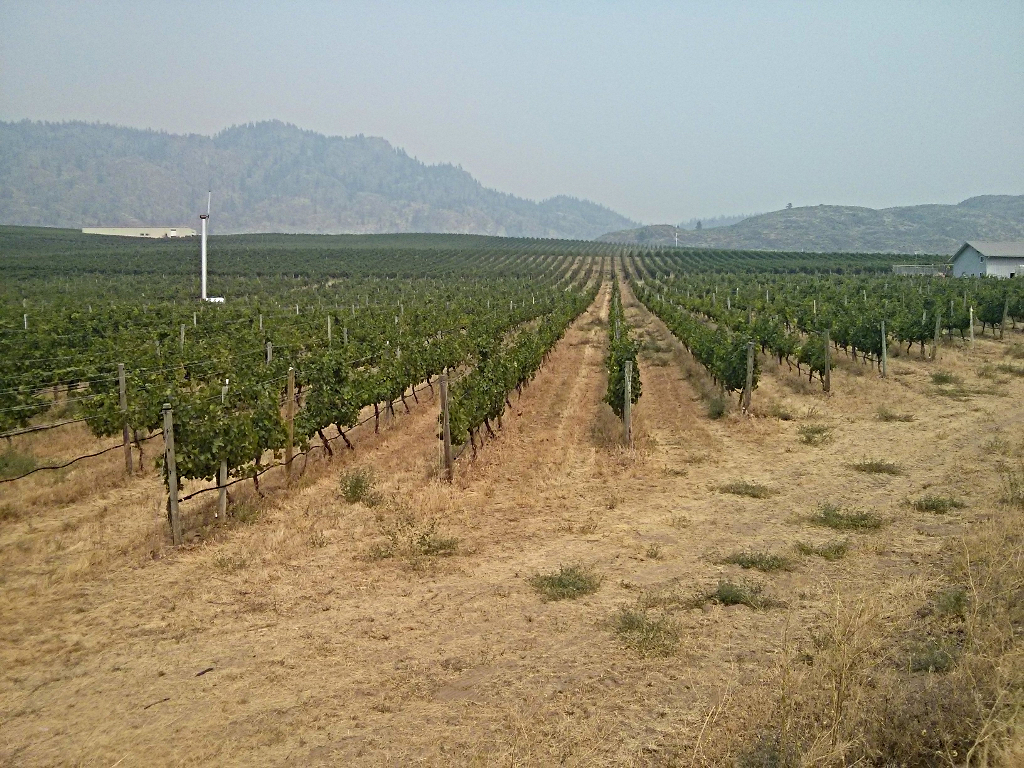
\includegraphics[width=1.0\linewidth]{tmp/photo_culmina_rows.pdf} 
\caption{Typical spacing of vinyard rows. Culmina Winery, Penticton, BC. August 2017.}
\label{fig:photo_culmina_rows}
\end{figure}

\begin{figure} %[htbp] % htbp stand for "here", "top", "bottom", "page"
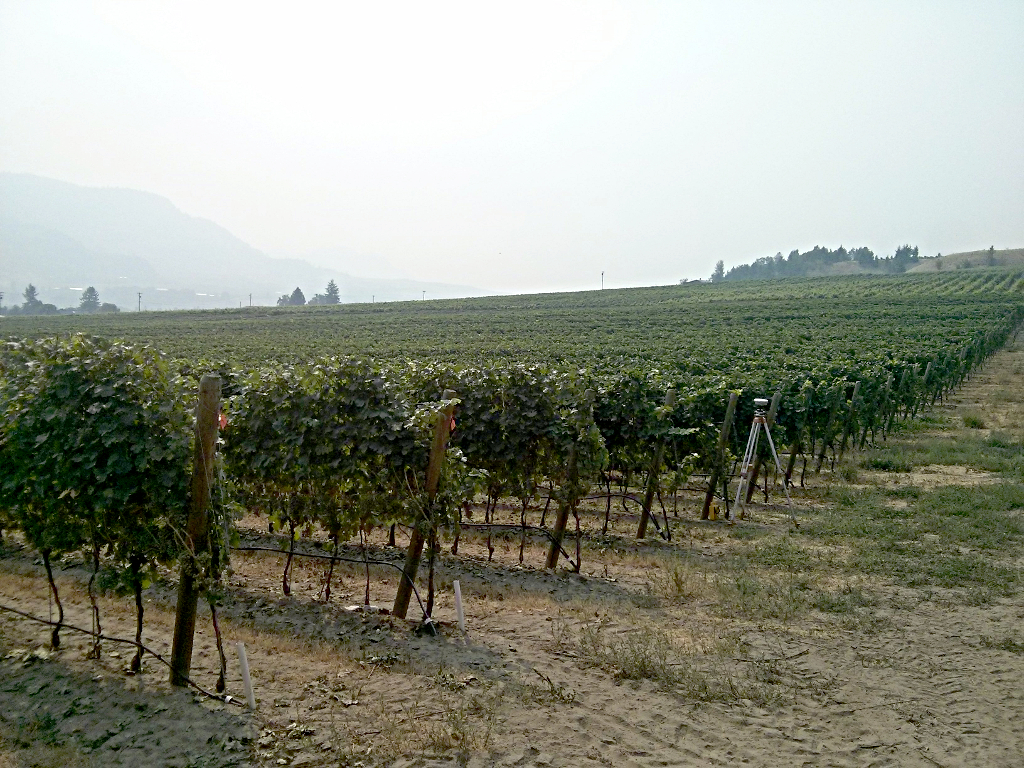
\includegraphics[width=1.0\linewidth]{tmp/photo_culmina_rows_slope.pdf} 
\caption{Low-frequency terrain variation, Culmina Winery, Penticton, BC. August 2017.}
\label{fig:photo_culmina_rows_slope}
\end{figure}

In the foregoing instances, a regular pattern of variation prevails, but there are other conditions that may confuse a system configured for these conditions. The subalpine regions of Canada's West Coast demonstrate the multi-scale variability, incoroporating smooth meadow-like environments, highly-variable multiple-aged forest canopies, and large-scale, high-relief terrain \ref{fig:photo_san_juan}.

\begin{figure} %[htbp] % htbp stand for "here", "top", "bottom", "page"
\begin{center}
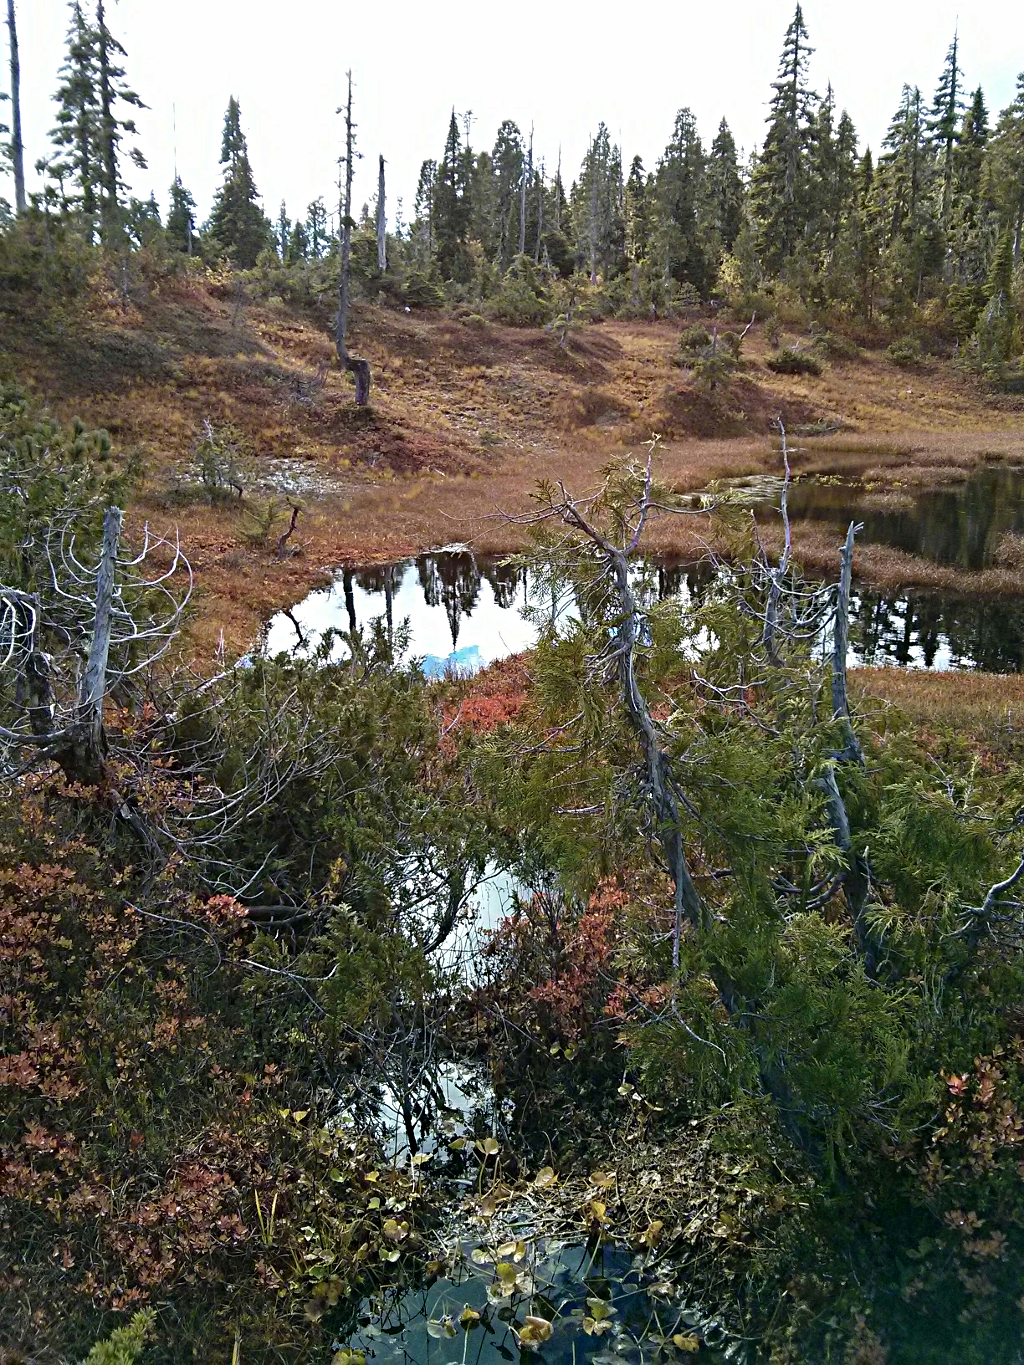
\includegraphics[width=0.5\linewidth]{tmp/photo_san_juan.pdf} 
\end{center}
\caption{Subalpine environment, San Juan Ridge, BC. October 2014.}
\label{fig:photo_san_juan}
\end{figure}

